\documentclass[twoside]{book}

% Packages required by doxygen
\usepackage{calc}
\usepackage{doxygen}
\usepackage{graphicx}
\usepackage[utf8]{inputenc}
\usepackage{makeidx}
\usepackage{multicol}
\usepackage{multirow}
\usepackage{textcomp}
\usepackage[table]{xcolor}

% NLS support packages
\usepackage{polski}
\usepackage[T1]{fontenc}

% Font selection
\usepackage[T1]{fontenc}
\usepackage{mathptmx}
\usepackage[scaled=.90]{helvet}
\usepackage{courier}
\usepackage{amssymb}
\usepackage{sectsty}
\renewcommand{\familydefault}{\sfdefault}
\allsectionsfont{%
  \fontseries{bc}\selectfont%
  \color{darkgray}%
}
\renewcommand{\DoxyLabelFont}{%
  \fontseries{bc}\selectfont%
  \color{darkgray}%
}

% Page & text layout
\usepackage{geometry}
\geometry{%
  a4paper,%
  top=2.5cm,%
  bottom=2.5cm,%
  left=2.5cm,%
  right=2.5cm%
}
\tolerance=750
\hfuzz=15pt
\hbadness=750
\setlength{\emergencystretch}{15pt}
\setlength{\parindent}{0cm}
\setlength{\parskip}{0.2cm}
\makeatletter
\renewcommand{\paragraph}{%
  \@startsection{paragraph}{4}{0ex}{-1.0ex}{1.0ex}{%
    \normalfont\normalsize\bfseries\SS@parafont%
  }%
}
\renewcommand{\subparagraph}{%
  \@startsection{subparagraph}{5}{0ex}{-1.0ex}{1.0ex}{%
    \normalfont\normalsize\bfseries\SS@subparafont%
  }%
}
\makeatother

% Headers & footers
\usepackage{fancyhdr}
\pagestyle{fancyplain}
\fancyhead[LE]{\fancyplain{}{\bfseries\thepage}}
\fancyhead[CE]{\fancyplain{}{}}
\fancyhead[RE]{\fancyplain{}{\bfseries\leftmark}}
\fancyhead[LO]{\fancyplain{}{\bfseries\rightmark}}
\fancyhead[CO]{\fancyplain{}{}}
\fancyhead[RO]{\fancyplain{}{\bfseries\thepage}}
\fancyfoot[LE]{\fancyplain{}{}}
\fancyfoot[CE]{\fancyplain{}{}}
\fancyfoot[RE]{\fancyplain{}{\bfseries\scriptsize Wygenerowano Wt, 19 maj 2015 14\-:17\-:55 dla P\-A\-M\-S\-I programem Doxygen }}
\fancyfoot[LO]{\fancyplain{}{\bfseries\scriptsize Wygenerowano Wt, 19 maj 2015 14\-:17\-:55 dla P\-A\-M\-S\-I programem Doxygen }}
\fancyfoot[CO]{\fancyplain{}{}}
\fancyfoot[RO]{\fancyplain{}{}}
\renewcommand{\footrulewidth}{0.4pt}
\renewcommand{\chaptermark}[1]{%
  \markboth{#1}{}%
}
\renewcommand{\sectionmark}[1]{%
  \markright{\thesection\ #1}%
}

% Indices & bibliography
\usepackage{natbib}
\usepackage[titles]{tocloft}
\setcounter{tocdepth}{3}
\setcounter{secnumdepth}{5}
\makeindex

% Hyperlinks (required, but should be loaded last)
\usepackage{ifpdf}
\ifpdf
  \usepackage[pdftex,pagebackref=true]{hyperref}
\else
  \usepackage[ps2pdf,pagebackref=true]{hyperref}
\fi
\hypersetup{%
  colorlinks=true,%
  linkcolor=blue,%
  citecolor=blue,%
  unicode%
}

% Custom commands
\newcommand{\clearemptydoublepage}{%
  \newpage{\pagestyle{empty}\cleardoublepage}%
}


%===== C O N T E N T S =====

\begin{document}

% Titlepage & ToC
\hypersetup{pageanchor=false}
\pagenumbering{roman}
\begin{titlepage}
\vspace*{7cm}
\begin{center}%
{\Large P\-A\-M\-S\-I \\[1ex]\large 0.\-1 }\\
\vspace*{1cm}
{\large Wygenerowano przez Doxygen 1.8.6}\\
\vspace*{0.5cm}
{\small Wt, 19 maj 2015 14:17:55}\\
\end{center}
\end{titlepage}
\clearemptydoublepage
\tableofcontents
\clearemptydoublepage
\pagenumbering{arabic}
\hypersetup{pageanchor=true}

%--- Begin generated contents ---
\chapter{Indeks hierarchiczny}
\section{Hierarchia klas}
Ta lista dziedziczenia posortowana jest z grubsza, choć nie całkowicie, alfabetycznie\-:\begin{DoxyCompactList}
\item \contentsline{section}{A\-B\-Data$<$ type $>$}{\pageref{class_a_b_data}}{}
\begin{DoxyCompactList}
\item \contentsline{section}{List$<$ type $>$}{\pageref{class_list}}{}
\item \contentsline{section}{List\-Array$<$ type $>$}{\pageref{class_list_array}}{}
\item \contentsline{section}{Queue$<$ type $>$}{\pageref{class_queue}}{}
\item \contentsline{section}{Stack$<$ type $>$}{\pageref{class_stack}}{}
\end{DoxyCompactList}
\item \contentsline{section}{A\-B\-Data$<$ Assoc\-Data$<$ type\-Key, type $>$ $>$}{\pageref{class_a_b_data}}{}
\begin{DoxyCompactList}
\item \contentsline{section}{List$<$ Assoc\-Data$<$ type\-Key, type $>$ $>$}{\pageref{class_list}}{}
\end{DoxyCompactList}
\item \contentsline{section}{A\-B\-Data$<$ Observer $\ast$ $>$}{\pageref{class_a_b_data}}{}
\begin{DoxyCompactList}
\item \contentsline{section}{Stack$<$ Observer $\ast$ $>$}{\pageref{class_stack}}{}
\end{DoxyCompactList}
\item \contentsline{section}{Assoc\-Data$<$ type\-Key, type $>$}{\pageref{struct_assoc_data}}{}
\item \contentsline{section}{Assoc\-Tab$<$ type\-Key, type $>$}{\pageref{class_assoc_tab}}{}
\item \contentsline{section}{Iterable$<$ type $>$}{\pageref{class_iterable}}{}
\begin{DoxyCompactList}
\item \contentsline{section}{List$<$ type $>$}{\pageref{class_list}}{}
\item \contentsline{section}{List\-Array$<$ type $>$}{\pageref{class_list_array}}{}
\item \contentsline{section}{Queue$<$ type $>$}{\pageref{class_queue}}{}
\item \contentsline{section}{Stack$<$ type $>$}{\pageref{class_stack}}{}
\end{DoxyCompactList}
\item \contentsline{section}{Iterable$<$ Assoc\-Data$<$ type\-Key, type $>$ $>$}{\pageref{class_iterable}}{}
\begin{DoxyCompactList}
\item \contentsline{section}{List$<$ Assoc\-Data$<$ type\-Key, type $>$ $>$}{\pageref{class_list}}{}
\end{DoxyCompactList}
\item \contentsline{section}{Iterable$<$ Observer $\ast$ $>$}{\pageref{class_iterable}}{}
\begin{DoxyCompactList}
\item \contentsline{section}{Stack$<$ Observer $\ast$ $>$}{\pageref{class_stack}}{}
\end{DoxyCompactList}
\item \contentsline{section}{node$<$ type $>$}{\pageref{structnode}}{}
\item \contentsline{section}{node$<$ Assoc\-Data$<$ type\-Key, type $>$ $>$}{\pageref{structnode}}{}
\item \contentsline{section}{node$<$ Observer $\ast$ $>$}{\pageref{structnode}}{}
\item \contentsline{section}{Observer}{\pageref{class_observer}}{}
\begin{DoxyCompactList}
\item \contentsline{section}{Save\-To\-File}{\pageref{class_save_to_file}}{}
\end{DoxyCompactList}
\item \contentsline{section}{Subject}{\pageref{class_subject}}{}
\begin{DoxyCompactList}
\item \contentsline{section}{Benchmark}{\pageref{class_benchmark}}{}
\end{DoxyCompactList}
\item \contentsline{section}{Timer}{\pageref{class_timer}}{}
\begin{DoxyCompactList}
\item \contentsline{section}{Benchmark}{\pageref{class_benchmark}}{}
\end{DoxyCompactList}
\end{DoxyCompactList}

\chapter{Indeks klas}
\section{Lista klas}
Tutaj znajdują się klasy, struktury, unie i interfejsy wraz z ich krótkimi opisami\-:\begin{DoxyCompactList}
\item\contentsline{section}{\hyperlink{class_a_b_data}{A\-B\-Data$<$ type $>$} \\*Modeluje klase wirtualna \hyperlink{class_a_b_data}{A\-B\-Data}, ktora jest interfejsem }{\pageref{class_a_b_data}}{}
\item\contentsline{section}{\hyperlink{struct_assoc_data}{Assoc\-Data$<$ type\-Key, type $>$} }{\pageref{struct_assoc_data}}{}
\item\contentsline{section}{\hyperlink{class_assoc_tab}{Assoc\-Tab$<$ type\-Key, type $>$} }{\pageref{class_assoc_tab}}{}
\item\contentsline{section}{\hyperlink{class_benchmark}{Benchmark} \\*Klasa \hyperlink{class_benchmark}{Benchmark} }{\pageref{class_benchmark}}{}
\item\contentsline{section}{\hyperlink{class_binary_tree}{Binary\-Tree$<$ type $>$} \\*Klasa \hyperlink{class_binary_tree}{Binary\-Tree} -\/ drzewo binarne }{\pageref{class_binary_tree}}{}
\item\contentsline{section}{\hyperlink{class_graph}{Graph} }{\pageref{class_graph}}{}
\item\contentsline{section}{\hyperlink{class_iterable}{Iterable$<$ type $>$} \\*Modeluje klase wirtualna \hyperlink{class_iterable}{Iterable} }{\pageref{class_iterable}}{}
\item\contentsline{section}{\hyperlink{class_list}{List$<$ type $>$} }{\pageref{class_list}}{}
\item\contentsline{section}{\hyperlink{class_list_array}{List\-Array$<$ type $>$} }{\pageref{class_list_array}}{}
\item\contentsline{section}{\hyperlink{structnode}{node$<$ type $>$} }{\pageref{structnode}}{}
\item\contentsline{section}{\hyperlink{class_observer}{Observer} }{\pageref{class_observer}}{}
\item\contentsline{section}{\hyperlink{class_queue}{Queue$<$ type $>$} }{\pageref{class_queue}}{}
\item\contentsline{section}{\hyperlink{structrbtreenode}{rbtreenode$<$ type $>$} }{\pageref{structrbtreenode}}{}
\item\contentsline{section}{\hyperlink{class_red_black_tree}{Red\-Black\-Tree$<$ type $>$} \\*Klasa \hyperlink{class_red_black_tree}{Red\-Black\-Tree} -\/ drzewo czerwono-\/czarne }{\pageref{class_red_black_tree}}{}
\item\contentsline{section}{\hyperlink{class_save_to_file}{Save\-To\-File} }{\pageref{class_save_to_file}}{}
\item\contentsline{section}{\hyperlink{class_stack}{Stack$<$ type $>$} }{\pageref{class_stack}}{}
\item\contentsline{section}{\hyperlink{class_subject}{Subject} }{\pageref{class_subject}}{}
\item\contentsline{section}{\hyperlink{class_timer}{Timer} }{\pageref{class_timer}}{}
\item\contentsline{section}{\hyperlink{structtreenode}{treenode$<$ type $>$} \\*Wezel drzewa }{\pageref{structtreenode}}{}
\item\contentsline{section}{\hyperlink{class_trees}{Trees$<$ type $>$} \\*Klasa abstrakcyjna zawierajaca metody wirtualne drzew }{\pageref{class_trees}}{}
\end{DoxyCompactList}

\chapter{Indeks plików}
\section{Lista plików}
Tutaj znajduje się lista wszystkich plików z ich krótkimi opisami\-:\begin{DoxyCompactList}
\item\contentsline{section}{\hyperlink{benchmark_8cpp}{benchmark.\-cpp} \\*Plik zawiera metody klasy \hyperlink{class_benchmark}{Benchmark} }{\pageref{benchmark_8cpp}}{}
\item\contentsline{section}{\hyperlink{benchmark_8hh}{benchmark.\-hh} \\*Definicja klasy \hyperlink{class_benchmark}{Benchmark} }{\pageref{benchmark_8hh}}{}
\item\contentsline{section}{\hyperlink{main_8cpp}{main.\-cpp} }{\pageref{main_8cpp}}{}
\item\contentsline{section}{\hyperlink{program_8cpp}{program.\-cpp} \\*Plik zawiera metody klasy \hyperlink{class_program}{Program} }{\pageref{program_8cpp}}{}
\item\contentsline{section}{\hyperlink{program_8hh}{program.\-hh} \\*Definicja klasy \hyperlink{class_program}{Program} }{\pageref{program_8hh}}{}
\item\contentsline{section}{\hyperlink{tabx2_8cpp}{tabx2.\-cpp} \\*Plik zawiera metody klasy \hyperlink{class_tabx2}{Tabx2} }{\pageref{tabx2_8cpp}}{}
\item\contentsline{section}{\hyperlink{tabx2_8hh}{tabx2.\-hh} \\*Definicja klasy \hyperlink{class_tabx2}{Tabx2} }{\pageref{tabx2_8hh}}{}
\end{DoxyCompactList}

\chapter{Dokumentacja klas}
\input{class_a_b_data}
\input{class_assoc_tab}
\hypertarget{class_benchmark}{\section{Dokumentacja klasy Benchmark}
\label{class_benchmark}\index{Benchmark@{Benchmark}}
}


Klasa \hyperlink{class_benchmark}{Benchmark}.  




{\ttfamily \#include $<$benchmark.\-hh$>$}

\subsection*{Metody publiczne}
\begin{DoxyCompactItemize}
\item 
void \hyperlink{class_benchmark_a684ddcbdd22608838da1ad23f1fcc2ce}{rozpocznij\-\_\-pomiar} ()
\begin{DoxyCompactList}\small\item\em Procedura rozpocznij\-\_\-pomiar. \end{DoxyCompactList}\item 
void \hyperlink{class_benchmark_a3f4b4595a3d1145d238f5b3c8486d875}{zakoncz\-\_\-pomiar} ()
\begin{DoxyCompactList}\small\item\em Procedura zakoncz\-\_\-pomiar. \end{DoxyCompactList}\item 
double \hyperlink{class_benchmark_ad2f9d4a8ee5a33de5261c2b2eff3d87a}{testuj} (\hyperlink{class_program}{Program} \&program, char $\ast$dane, int ilosc\-\_\-danych, int ilosc\-\_\-testow)
\begin{DoxyCompactList}\small\item\em Metoda testuj. \end{DoxyCompactList}\end{DoxyCompactItemize}
\subsection*{Atrybuty prywatne}
\begin{DoxyCompactItemize}
\item 
timeval \hyperlink{class_benchmark_ab951e55dc4470926e0eb0761804f13bc}{t1}
\begin{DoxyCompactList}\small\item\em Zmienne t1, t2. \end{DoxyCompactList}\item 
timeval \hyperlink{class_benchmark_a2b145dd2458fea33d6df41f310058bec}{t2}
\item 
double \hyperlink{class_benchmark_ab72b3cbe324970fd8c738f03718d52fc}{czas\-\_\-pomiaru}
\begin{DoxyCompactList}\small\item\em Zmienna czas\-\_\-pomiaru. \end{DoxyCompactList}\end{DoxyCompactItemize}


\subsection{Opis szczegółowy}
Jest to klasa służąca do testowania programów. 

Definicja w linii \hyperlink{benchmark_8hh_source_l00023}{23} pliku \hyperlink{benchmark_8hh_source}{benchmark.\-hh}.



\subsection{Dokumentacja funkcji składowych}
\hypertarget{class_benchmark_a684ddcbdd22608838da1ad23f1fcc2ce}{\index{Benchmark@{Benchmark}!rozpocznij\-\_\-pomiar@{rozpocznij\-\_\-pomiar}}
\index{rozpocznij\-\_\-pomiar@{rozpocznij\-\_\-pomiar}!Benchmark@{Benchmark}}
\subsubsection[{rozpocznij\-\_\-pomiar}]{\setlength{\rightskip}{0pt plus 5cm}void Benchmark\-::rozpocznij\-\_\-pomiar (
\begin{DoxyParamCaption}
{}
\end{DoxyParamCaption}
)}}\label{class_benchmark_a684ddcbdd22608838da1ad23f1fcc2ce}
Rozpoczyna pomiar czasu. 

Definicja w linii \hyperlink{benchmark_8cpp_source_l00007}{7} pliku \hyperlink{benchmark_8cpp_source}{benchmark.\-cpp}.



Oto graf wywoływań tej funkcji\-:
\nopagebreak
\begin{figure}[H]
\begin{center}
\leavevmode
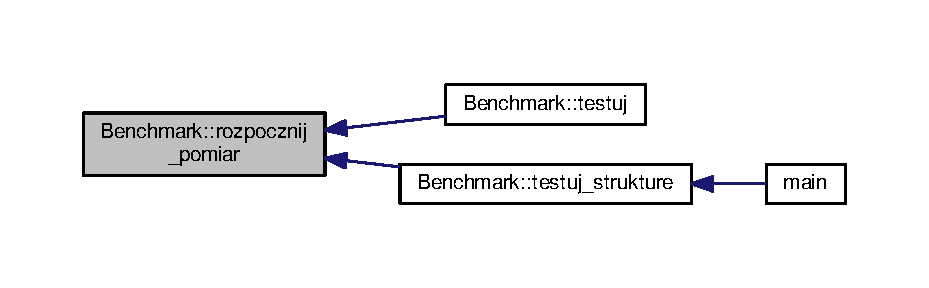
\includegraphics[width=350pt]{class_benchmark_a684ddcbdd22608838da1ad23f1fcc2ce_icgraph}
\end{center}
\end{figure}


\hypertarget{class_benchmark_ad2f9d4a8ee5a33de5261c2b2eff3d87a}{\index{Benchmark@{Benchmark}!testuj@{testuj}}
\index{testuj@{testuj}!Benchmark@{Benchmark}}
\subsubsection[{testuj}]{\setlength{\rightskip}{0pt plus 5cm}double Benchmark\-::testuj (
\begin{DoxyParamCaption}
\item[{{\bf Program} \&}]{program, }
\item[{char $\ast$}]{dane, }
\item[{int}]{ilosc\-\_\-danych, }
\item[{int}]{ilosc\-\_\-testow}
\end{DoxyParamCaption}
)}}\label{class_benchmark_ad2f9d4a8ee5a33de5261c2b2eff3d87a}
Dokonuje testow wybranego programu.


\begin{DoxyParams}[1]{Parametry}
\mbox{\tt in}  & {\em program} & \hyperlink{class_program}{Program} wybrany do testowania. \\
\hline
\mbox{\tt in}  & {\em dane} & Wskaznik na nazwe pliku z danymi. \\
\hline
\mbox{\tt in}  & {\em ilosc\-\_\-danych} & Ilosc danych, ktore chcemy pobrac do testu. \\
\hline
\mbox{\tt in}  & {\em ilosc\-\_\-testow} & Ilosc testow, jakie chcemy przeprowadzic.\\
\hline
\end{DoxyParams}
\begin{DoxyReturn}{Zwraca}
Metoda zwraca sredni czas wykonania programu dla podanych parametrow. 
\end{DoxyReturn}


Definicja w linii \hyperlink{benchmark_8cpp_source_l00017}{17} pliku \hyperlink{benchmark_8cpp_source}{benchmark.\-cpp}.



Oto graf wywołań dla tej funkcji\-:
\nopagebreak
\begin{figure}[H]
\begin{center}
\leavevmode
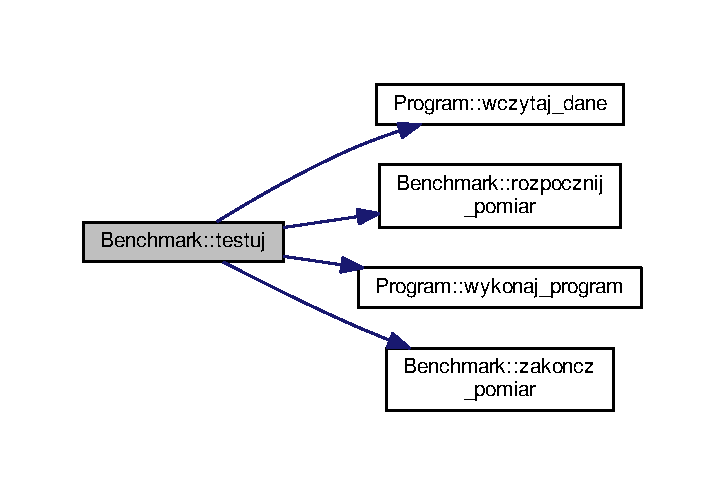
\includegraphics[width=348pt]{class_benchmark_ad2f9d4a8ee5a33de5261c2b2eff3d87a_cgraph}
\end{center}
\end{figure}




Oto graf wywoływań tej funkcji\-:
\nopagebreak
\begin{figure}[H]
\begin{center}
\leavevmode
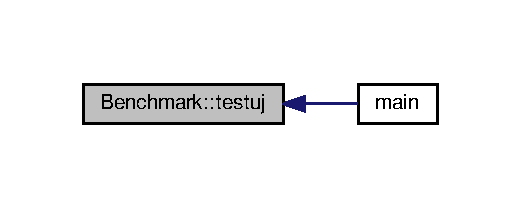
\includegraphics[width=250pt]{class_benchmark_ad2f9d4a8ee5a33de5261c2b2eff3d87a_icgraph}
\end{center}
\end{figure}


\hypertarget{class_benchmark_a3f4b4595a3d1145d238f5b3c8486d875}{\index{Benchmark@{Benchmark}!zakoncz\-\_\-pomiar@{zakoncz\-\_\-pomiar}}
\index{zakoncz\-\_\-pomiar@{zakoncz\-\_\-pomiar}!Benchmark@{Benchmark}}
\subsubsection[{zakoncz\-\_\-pomiar}]{\setlength{\rightskip}{0pt plus 5cm}void Benchmark\-::zakoncz\-\_\-pomiar (
\begin{DoxyParamCaption}
{}
\end{DoxyParamCaption}
)}}\label{class_benchmark_a3f4b4595a3d1145d238f5b3c8486d875}
Konczy pomiar czasu i zapisuje wartosc zmierzona w zmiennej czas\-\_\-pomiaru. 

Definicja w linii \hyperlink{benchmark_8cpp_source_l00011}{11} pliku \hyperlink{benchmark_8cpp_source}{benchmark.\-cpp}.



Oto graf wywoływań tej funkcji\-:
\nopagebreak
\begin{figure}[H]
\begin{center}
\leavevmode
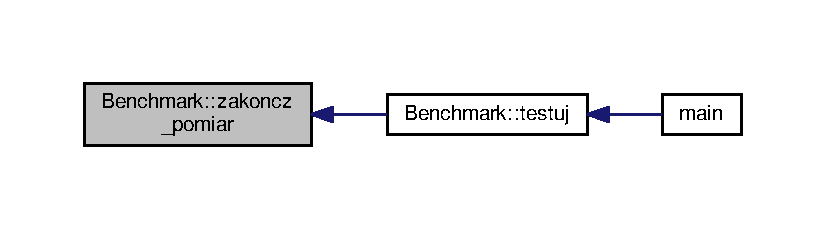
\includegraphics[width=350pt]{class_benchmark_a3f4b4595a3d1145d238f5b3c8486d875_icgraph}
\end{center}
\end{figure}




\subsection{Dokumentacja atrybutów składowych}
\hypertarget{class_benchmark_ab72b3cbe324970fd8c738f03718d52fc}{\index{Benchmark@{Benchmark}!czas\-\_\-pomiaru@{czas\-\_\-pomiaru}}
\index{czas\-\_\-pomiaru@{czas\-\_\-pomiaru}!Benchmark@{Benchmark}}
\subsubsection[{czas\-\_\-pomiaru}]{\setlength{\rightskip}{0pt plus 5cm}double Benchmark\-::czas\-\_\-pomiaru\hspace{0.3cm}{\ttfamily [private]}}}\label{class_benchmark_ab72b3cbe324970fd8c738f03718d52fc}
Przechowuje obliczony czas pojedynczego pomiaru (w ms) 

Definicja w linii \hyperlink{benchmark_8hh_source_l00037}{37} pliku \hyperlink{benchmark_8hh_source}{benchmark.\-hh}.

\hypertarget{class_benchmark_ab951e55dc4470926e0eb0761804f13bc}{\index{Benchmark@{Benchmark}!t1@{t1}}
\index{t1@{t1}!Benchmark@{Benchmark}}
\subsubsection[{t1}]{\setlength{\rightskip}{0pt plus 5cm}timeval Benchmark\-::t1\hspace{0.3cm}{\ttfamily [private]}}}\label{class_benchmark_ab951e55dc4470926e0eb0761804f13bc}
Zmienne przechowujace momenty rozpaczecia i zakonczenia pomiaru czasu. 

Definicja w linii \hyperlink{benchmark_8hh_source_l00030}{30} pliku \hyperlink{benchmark_8hh_source}{benchmark.\-hh}.

\hypertarget{class_benchmark_a2b145dd2458fea33d6df41f310058bec}{\index{Benchmark@{Benchmark}!t2@{t2}}
\index{t2@{t2}!Benchmark@{Benchmark}}
\subsubsection[{t2}]{\setlength{\rightskip}{0pt plus 5cm}timeval Benchmark\-::t2\hspace{0.3cm}{\ttfamily [private]}}}\label{class_benchmark_a2b145dd2458fea33d6df41f310058bec}


Definicja w linii \hyperlink{benchmark_8hh_source_l00030}{30} pliku \hyperlink{benchmark_8hh_source}{benchmark.\-hh}.



Dokumentacja dla tej klasy została wygenerowana z plików\-:\begin{DoxyCompactItemize}
\item 
\hyperlink{benchmark_8hh}{benchmark.\-hh}\item 
\hyperlink{benchmark_8cpp}{benchmark.\-cpp}\end{DoxyCompactItemize}

\input{struct_assoc_tab_1_1_data}
\input{class_iterable}
\input{class_list}
\input{class_list_array}
\input{structnode}
\input{class_observer}
\input{class_queue}
\input{class_save_to_file}
\input{class_stack}
\input{class_subject}
\input{class_timer}
\chapter{Dokumentacja plików}
\input{abdata_8hh}
\input{abdata_8hh_source}
\input{abdatatools_8hh}
\input{abdatatools_8hh_source}
\input{assoctab_8hh}
\input{assoctab_8hh_source}
\hypertarget{benchmark_8cpp}{\section{Dokumentacja pliku benchmark.\-cpp}
\label{benchmark_8cpp}\index{benchmark.\-cpp@{benchmark.\-cpp}}
}


Plik zawiera metody klasy \hyperlink{class_benchmark}{Benchmark}.  


{\ttfamily \#include \char`\"{}benchmark.\-hh\char`\"{}}\\*
Wykres zależności załączania dla benchmark.\-cpp\-:\nopagebreak
\begin{figure}[H]
\begin{center}
\leavevmode
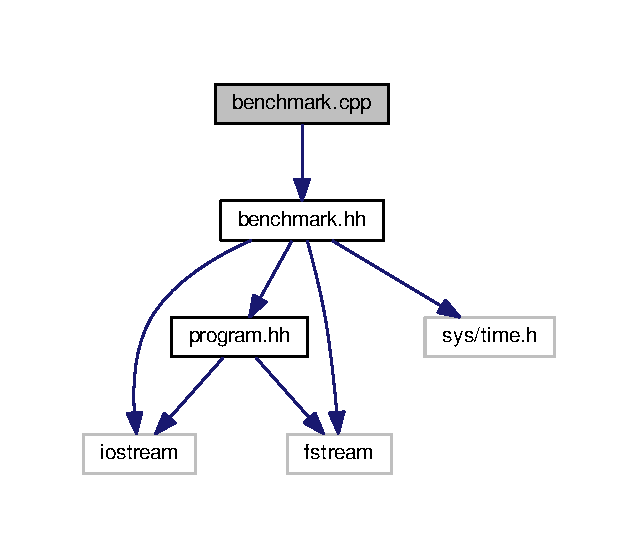
\includegraphics[width=306pt]{benchmark_8cpp__incl}
\end{center}
\end{figure}

\hypertarget{benchmark_8cpp}{\section{benchmark.\-cpp}
\label{benchmark_8cpp}\index{benchmark.\-cpp@{benchmark.\-cpp}}
}

\begin{DoxyCode}
00001 \textcolor{preprocessor}{#include "\hyperlink{benchmark_8hh}{Benchmark/benchmark.hh}"}
00002 \textcolor{preprocessor}{#include <cstdlib>}
00003 \textcolor{preprocessor}{#include <iostream>}
\hypertarget{benchmark_8cpp_source_l00008}{}\hyperlink{class_benchmark_a408a44a1d64e45b647ef6dbba2f2c3d3}{00008} \textcolor{keywordtype}{void} \hyperlink{class_benchmark_a408a44a1d64e45b647ef6dbba2f2c3d3}{Benchmark::notify}()\{
00009   \textcolor{keywordflow}{for}(\textcolor{keywordtype}{unsigned} \textcolor{keywordtype}{int} i=0; i<\hyperlink{class_subject_ad8f878ad28617e54691c4f74cd84cbe0}{obss}.\hyperlink{class_stack_a0d5ba9f716bd2c43a07cc638b8ee166f}{size}();i++)
00010     \hyperlink{class_subject_ad8f878ad28617e54691c4f74cd84cbe0}{obss}[i]->update(\hyperlink{class_benchmark_a1d0eaa6febe9b7a7f5f5147e83f60910}{amount}, \hyperlink{class_benchmark_aa88092b6164ad7d1243162d3012f729a}{mean});
00011 \}
00012 
\hypertarget{benchmark_8cpp_source_l00013}{}\hyperlink{class_benchmark_ab65889d4c2df3eb503048ab1cc6e7413}{00013} \textcolor{keywordtype}{void} \hyperlink{class_benchmark_ab65889d4c2df3eb503048ab1cc6e7413}{Benchmark::stop\_Ctimer}()\{
00014   \hyperlink{class_timer_ac05cde2d44f1a1fc40554bf78a65fe0e}{stop\_timer}();
00015   \hyperlink{class_benchmark_a7130c0718e3a3ab2fea70285dab122a2}{total}+=\hyperlink{class_timer_ab07af01194380dc8df3f3791f9aa803a}{atime};
00016   \hyperlink{class_benchmark_a3a56c7dad0b21e490f3024d5d0027f31}{counter}++;
00017 \}
00018 
\hypertarget{benchmark_8cpp_source_l00019}{}\hyperlink{class_benchmark_ac4d5360d2850510913efe07cf957f4c1}{00019} \textcolor{keywordtype}{void} \hyperlink{class_benchmark_ac4d5360d2850510913efe07cf957f4c1}{Benchmark::calc\_mean}()\{
00020   \hyperlink{class_benchmark_aa88092b6164ad7d1243162d3012f729a}{mean}=\hyperlink{class_benchmark_a7130c0718e3a3ab2fea70285dab122a2}{total}/\hyperlink{class_benchmark_a3a56c7dad0b21e490f3024d5d0027f31}{counter};
00021   std::cout << \hyperlink{class_benchmark_aa88092b6164ad7d1243162d3012f729a}{mean} << \textcolor{stringliteral}{"  "} << \hyperlink{class_benchmark_a1d0eaa6febe9b7a7f5f5147e83f60910}{amount} << \textcolor{stringliteral}{"    "} << std::endl;
00022   \hyperlink{class_benchmark_a408a44a1d64e45b647ef6dbba2f2c3d3}{notify}();
00023 \}
00024 
00025 \textcolor{keyword}{template}<\textcolor{keyword}{typename} type>
\hypertarget{benchmark_8cpp_source_l00026}{}\hyperlink{class_benchmark_ad5d8a563d9b9163758ae04d064cc38cb}{00026} \textcolor{keywordtype}{void} \hyperlink{class_benchmark_ad5d8a563d9b9163758ae04d064cc38cb}{Benchmark::runBenchmarkSort}(\textcolor{keywordtype}{void} (*f)(
      \hyperlink{class_iterable}{Iterable<type>}&, \textcolor{keywordtype}{int}, \textcolor{keywordtype}{int}), \hyperlink{class_iterable}{Iterable<type>} &container, \textcolor{keywordtype}{int} dataCount, \textcolor{keywordtype}{int} 
      repeats)\{
00027   \hyperlink{class_benchmark_a1d0eaa6febe9b7a7f5f5147e83f60910}{amount} = dataCount;
00028   \hyperlink{class_benchmark_a7130c0718e3a3ab2fea70285dab122a2}{total}=0; 
00029   \hyperlink{class_benchmark_aa88092b6164ad7d1243162d3012f729a}{mean}=0;
00030   \hyperlink{class_benchmark_a3a56c7dad0b21e490f3024d5d0027f31}{counter}=0;
00031   \textcolor{keywordflow}{for}(\textcolor{keywordtype}{int} i=1; i<=repeats; i++)\{
00032     \hyperlink{class_timer_a83d4b873e3275a61004b5679672045c0}{start\_timer}();
00033     (*f)(container, 0, \hyperlink{class_benchmark_a1d0eaa6febe9b7a7f5f5147e83f60910}{amount}-1);
00034     \hyperlink{class_benchmark_ab65889d4c2df3eb503048ab1cc6e7413}{stop\_Ctimer}();
00035   \}
00036   \hyperlink{class_benchmark_ac4d5360d2850510913efe07cf957f4c1}{calc\_mean}();
00037 \}
00038 
\hypertarget{benchmark_8cpp_source_l00039}{}\hyperlink{class_benchmark_ae9e23e7f4cf294fad57f5c98298bf874}{00039} \textcolor{keywordtype}{void} \hyperlink{class_benchmark_ae9e23e7f4cf294fad57f5c98298bf874}{Benchmark::runBenchmarkSearchGraph}(\textcolor{keywordtype}{void} (
      \hyperlink{class_graph}{Graph}::*f)(), \hyperlink{class_graph}{Graph} graph, \textcolor{keywordtype}{int} dataCount, \textcolor{keywordtype}{int} repeats)\{
00040   \hyperlink{class_benchmark_a1d0eaa6febe9b7a7f5f5147e83f60910}{amount} = dataCount;
00041   \hyperlink{class_benchmark_a7130c0718e3a3ab2fea70285dab122a2}{total}=0; 
00042   \hyperlink{class_benchmark_aa88092b6164ad7d1243162d3012f729a}{mean}=0;
00043   \hyperlink{class_benchmark_a3a56c7dad0b21e490f3024d5d0027f31}{counter}=0;
00044 
00045   \textcolor{comment}{/* DANE - spojny losowy (*/}
00046   \textcolor{keywordflow}{if}(dataCount>1)
00047     graph.\hyperlink{class_graph_a98e8eaa5f6a140aefc67a9bf07023c27}{insertE}(0, 1);
00048   \textcolor{keywordflow}{for}(\textcolor{keywordtype}{int} j=1; j<dataCount; j++)
00049     graph.\hyperlink{class_graph_a98e8eaa5f6a140aefc67a9bf07023c27}{insertE}(j, rand()%j);
00050   \textcolor{comment}{/* DANE - 0 ze wszystkimi }
00051 \textcolor{comment}{     for(int j=0; j<dataCount; j++)}
00052 \textcolor{comment}{     graph.insertE(0,j);*/}
00053   \textcolor{comment}{/* DANE - LISTA }
00054 \textcolor{comment}{     for(int j=0; j<=dataCount-2; j++)\{}
00055 \textcolor{comment}{     graph.insertE(j, j+1);}
00056 \textcolor{comment}{     \}*/}
00057   \textcolor{keywordflow}{for}(\textcolor{keywordtype}{int} i=1; i<=repeats; i++)\{
00058     \hyperlink{class_timer_a83d4b873e3275a61004b5679672045c0}{start\_timer}();
00059     (graph.*f)();
00060     \hyperlink{class_benchmark_ab65889d4c2df3eb503048ab1cc6e7413}{stop\_Ctimer}();
00061   \}
00062   \hyperlink{class_benchmark_ac4d5360d2850510913efe07cf957f4c1}{calc\_mean}();
00063 \}
00064 
00065 
00066 
\end{DoxyCode}

\hypertarget{benchmark_8hh}{\section{Dokumentacja pliku benchmark.\-hh}
\label{benchmark_8hh}\index{benchmark.\-hh@{benchmark.\-hh}}
}


Definicja klasy \hyperlink{class_benchmark}{Benchmark}.  


{\ttfamily \#include $<$iostream$>$}\\*
{\ttfamily \#include \char`\"{}program.\-hh\char`\"{}}\\*
{\ttfamily \#include $<$sys/time.\-h$>$}\\*
{\ttfamily \#include $<$fstream$>$}\\*
Wykres zależności załączania dla benchmark.\-hh\-:
\nopagebreak
\begin{figure}[H]
\begin{center}
\leavevmode
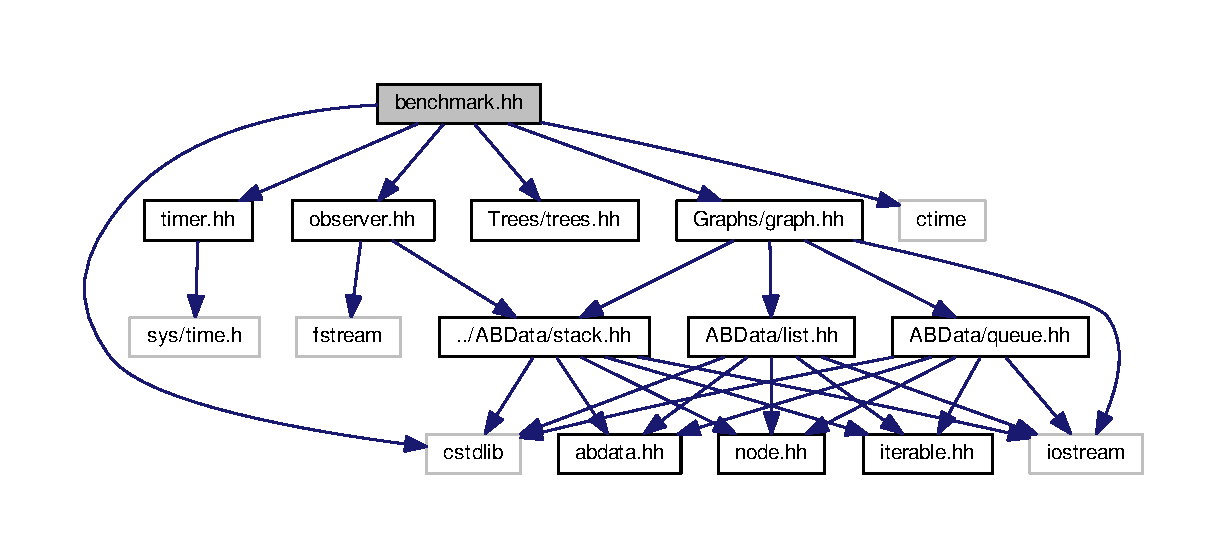
\includegraphics[width=306pt]{benchmark_8hh__incl}
\end{center}
\end{figure}
Ten wykres pokazuje, które pliki bezpośrednio lub pośrednio załączają ten plik\-:\nopagebreak
\begin{figure}[H]
\begin{center}
\leavevmode
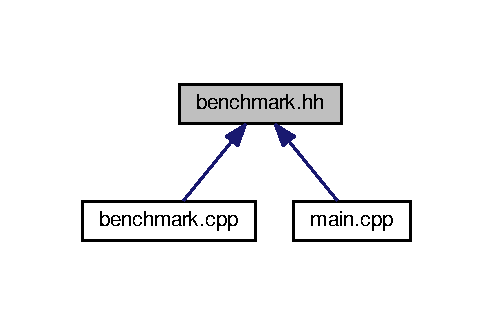
\includegraphics[width=237pt]{benchmark_8hh__dep__incl}
\end{center}
\end{figure}
\subsection*{Komponenty}
\begin{DoxyCompactItemize}
\item 
class \hyperlink{class_benchmark}{Benchmark}
\begin{DoxyCompactList}\small\item\em Klasa \hyperlink{class_benchmark}{Benchmark}. \end{DoxyCompactList}\end{DoxyCompactItemize}

\hypertarget{benchmark_8hh}{\section{benchmark.\-hh}
\label{benchmark_8hh}\index{benchmark.\-hh@{benchmark.\-hh}}
}

\begin{DoxyCode}
00001 \textcolor{comment}{//benchmark.hh}
00002 
00003 \textcolor{preprocessor}{#ifndef BENCHMARK\_HH}
00004 \textcolor{preprocessor}{}\textcolor{preprocessor}{#define BENCHMARK\_HH}
00005 \textcolor{preprocessor}{}
00006 \textcolor{preprocessor}{#include <iostream>}
00007 \textcolor{preprocessor}{#include "\hyperlink{program_8hh}{program.hh}"}
00008 \textcolor{preprocessor}{#include <sys/time.h>}
00009 \textcolor{preprocessor}{#include <fstream>}
00010 
00016 \textcolor{keyword}{using namespace }std;
00017 
\hypertarget{benchmark_8hh_source_l00023}{}\hyperlink{class_benchmark}{00023} \textcolor{keyword}{class }\hyperlink{class_benchmark}{Benchmark}\{
00024 \textcolor{keyword}{private}:
\hypertarget{benchmark_8hh_source_l00030}{}\hyperlink{class_benchmark_a2b145dd2458fea33d6df41f310058bec}{00030}   timeval t1, \hyperlink{class_benchmark_a2b145dd2458fea33d6df41f310058bec}{t2};
00031 
\hypertarget{benchmark_8hh_source_l00037}{}\hyperlink{class_benchmark_ab72b3cbe324970fd8c738f03718d52fc}{00037}   \textcolor{keywordtype}{double} \hyperlink{class_benchmark_ab72b3cbe324970fd8c738f03718d52fc}{czas\_pomiaru};
00038 
00039 \textcolor{keyword}{public}:
00045   \textcolor{keywordtype}{void} rozpocznij\_pomiar();
00046 
00052   \textcolor{keywordtype}{void} zakoncz\_pomiar();
00053 
00066   \textcolor{keywordtype}{double} testuj(\hyperlink{class_program}{Program} &program,\textcolor{keywordtype}{char}* dane, \textcolor{keywordtype}{int} ilosc\_danych, \textcolor{keywordtype}{int} ilosc\_testow);
00067 
00081   \textcolor{keywordtype}{double} testuj\_strukture(\hyperlink{class_program}{Program} &program,\textcolor{keywordtype}{char}* dane, \textcolor{keywordtype}{int} ilosc\_danych, \textcolor{keywordtype}{int} ilosc\_testow);
00082 \};
00083 
00084 \textcolor{preprocessor}{#endif}
\end{DoxyCode}

\input{iterable_8hh}
\input{iterable_8hh_source}
\input{list_8hh}
\input{list_8hh_source}
\input{listarray_8hh}
\input{listarray_8hh_source}
\hypertarget{main_8cpp}{\section{Dokumentacja pliku main.\-cpp}
\label{main_8cpp}\index{main.\-cpp@{main.\-cpp}}
}
{\ttfamily \#include \char`\"{}A\-B\-Data/list.\-hh\char`\"{}}\\*
{\ttfamily \#include \char`\"{}A\-B\-Data/stack.\-hh\char`\"{}}\\*
{\ttfamily \#include \char`\"{}A\-B\-Data/queue.\-hh\char`\"{}}\\*
{\ttfamily \#include \char`\"{}A\-B\-Data/iterable.\-hh\char`\"{}}\\*
{\ttfamily \#include \char`\"{}Benchmark/timer.\-hh\char`\"{}}\\*
{\ttfamily \#include \char`\"{}Benchmark/benchmark.\-hh\char`\"{}}\\*
{\ttfamily \#include \char`\"{}Benchmark/observer.\-hh\char`\"{}}\\*
{\ttfamily \#include \char`\"{}Trees/binarytree.\-hh\char`\"{}}\\*
{\ttfamily \#include \char`\"{}A\-B\-Data/sorts.\-hh\char`\"{}}\\*
{\ttfamily \#include \char`\"{}A\-B\-Data/abdatatools.\-hh\char`\"{}}\\*
{\ttfamily \#include \char`\"{}A\-B\-Data/listarray.\-hh\char`\"{}}\\*
{\ttfamily \#include \char`\"{}assoctab.\-hh\char`\"{}}\\*
{\ttfamily \#include \char`\"{}Trees/redblacktree.\-hh\char`\"{}}\\*
{\ttfamily \#include \char`\"{}unistd.\-h\char`\"{}}\\*
Wykres zależności załączania dla main.\-cpp\-:
\nopagebreak
\begin{figure}[H]
\begin{center}
\leavevmode
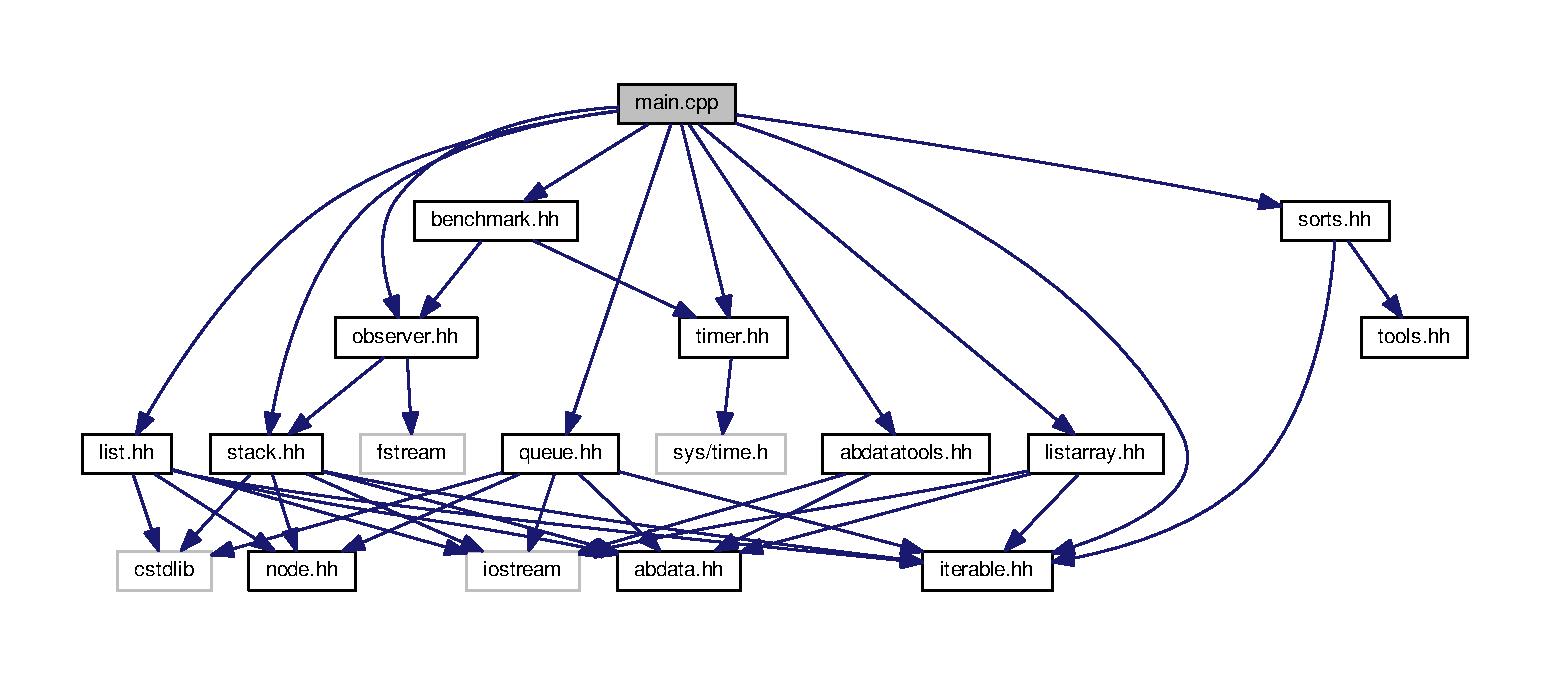
\includegraphics[width=350pt]{main_8cpp__incl}
\end{center}
\end{figure}
\subsection*{Funkcje}
\begin{DoxyCompactItemize}
\item 
int \hyperlink{main_8cpp_ae66f6b31b5ad750f1fe042a706a4e3d4}{main} ()
\end{DoxyCompactItemize}


\subsection{Dokumentacja funkcji}
\hypertarget{main_8cpp_ae66f6b31b5ad750f1fe042a706a4e3d4}{\index{main.\-cpp@{main.\-cpp}!main@{main}}
\index{main@{main}!main.cpp@{main.\-cpp}}
\subsubsection[{main}]{\setlength{\rightskip}{0pt plus 5cm}int main (
\begin{DoxyParamCaption}
{}
\end{DoxyParamCaption}
)}}\label{main_8cpp_ae66f6b31b5ad750f1fe042a706a4e3d4}


Definicja w linii \hyperlink{main_8cpp_source_l00018}{18} pliku \hyperlink{main_8cpp_source}{main.\-cpp}.



Oto graf wywołań dla tej funkcji\-:
\nopagebreak
\begin{figure}[H]
\begin{center}
\leavevmode
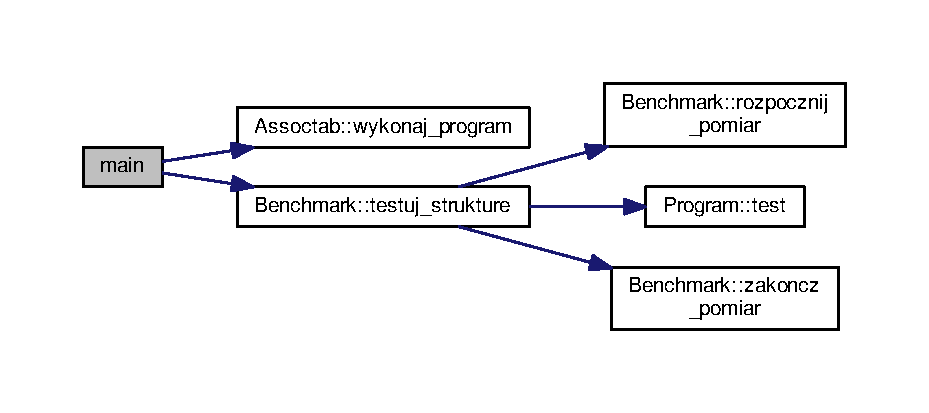
\includegraphics[width=350pt]{main_8cpp_ae66f6b31b5ad750f1fe042a706a4e3d4_cgraph}
\end{center}
\end{figure}



\hypertarget{main_8cpp}{\section{main.\-cpp}
\label{main_8cpp}\index{main.\-cpp@{main.\-cpp}}
}

\begin{DoxyCode}
00001 \textcolor{comment}{//main.cpp}
00002 \textcolor{preprocessor}{#include <iostream>}
00003 \textcolor{preprocessor}{#include "\hyperlink{program_8hh}{program.hh}"}
00004 \textcolor{preprocessor}{#include "\hyperlink{tabx2_8hh}{tabx2.hh}"}
00005 \textcolor{preprocessor}{#include "\hyperlink{benchmark_8hh}{benchmark.hh}"}
00006 \textcolor{preprocessor}{#include "\hyperlink{lista_8hh}{lista.hh}"}
00007 \textcolor{preprocessor}{#include "\hyperlink{lista__tab_8hh}{lista\_tab.hh}"}
00008 \textcolor{preprocessor}{#include "\hyperlink{assoctab_8hh}{assoctab.hh}"}
00009 
00010 \textcolor{keyword}{using namespace }std;
00011 
\hypertarget{main_8cpp_source_l00012}{}\hyperlink{main_8cpp_ae66f6b31b5ad750f1fe042a706a4e3d4}{00012} \textcolor{keywordtype}{int} \hyperlink{main_8cpp_ae66f6b31b5ad750f1fe042a706a4e3d4}{main}()\{
00013   \hyperlink{class_lista__tab}{Lista\_tab} a;
00014   \hyperlink{class_benchmark}{Benchmark} b;
00015   \textcolor{keywordtype}{char}* dane = (\textcolor{keywordtype}{char}*)\textcolor{stringliteral}{"dane.dat"};
00016   \textcolor{keywordtype}{int} ilosc\_testow = 10;
00017   
00018     a.\hyperlink{class_lista__tab_ac9adc6ecc7348c5e1871b239c1313405}{wykonaj\_program}(dane, 10);
00019     \textcolor{keywordflow}{for}(\textcolor{keywordtype}{int} i=0; i<=a.\hyperlink{class_lista__tab_afd2c6ba3ae15e658890641b188c7ed39}{iterator}; i++)
00020     cout<< a.\hyperlink{class_lista__tab_a123dfb670e5a5592e512c41cc4faf14e}{tab}[i]<<endl;
00021     a.\hyperlink{class_lista__tab_a409e9a4edbef4337980c7184b6cbfb63}{mergesort}(0,a.\hyperlink{class_lista__tab_afd2c6ba3ae15e658890641b188c7ed39}{iterator});
00022     cout<<endl<<endl;
00023     \textcolor{keywordflow}{for}(\textcolor{keywordtype}{int} i=0; i<=a.\hyperlink{class_lista__tab_afd2c6ba3ae15e658890641b188c7ed39}{iterator}; i++)
00024     cout<< a.\hyperlink{class_lista__tab_a123dfb670e5a5592e512c41cc4faf14e}{tab}[i]<<endl;
00025   
00026   \textcolor{comment}{/*}
00027 \textcolor{comment}{  for(int ilosc\_danych=1; ilosc\_danych<=10000000;ilosc\_danych*=10)\{}
00028 \textcolor{comment}{    cout << b.testuj\_strukture(a,dane,ilosc\_danych,ilosc\_testow) << endl;}
00029 \textcolor{comment}{  \}}
00030 \textcolor{comment}{  */}  
00031   \textcolor{keywordflow}{return} 0;
00032 \}
\end{DoxyCode}

\input{node_8hh}
\input{node_8hh_source}
\input{observer_8hh}
\input{observer_8hh_source}
\input{queue_8hh}
\input{queue_8hh_source}
\input{sorts_8hh}
\input{sorts_8hh_source}
\input{stack_8hh}
\input{stack_8hh_source}
\input{timer_8cpp}
\input{timer_8cpp_source}
\input{timer_8hh}
\input{timer_8hh_source}
\input{tools_8hh}
\input{tools_8hh_source}
%--- End generated contents ---

% Index
\newpage
\phantomsection
\addcontentsline{toc}{chapter}{Indeks}
\printindex

\end{document}
